\section{Experiments}
\label{sec:experiment}
%\KZ{Give a little preamble here.}
In this section, we discuss some end-to-end experimental results 
comparing ChatMatch (CM) and some baseline methods. 
We also show some ablation studies with different settings of 
CM.

\subsection{Experiment Settings}

\subsubsection*{Description of Seven Bots}
%\KZ{Put these and the next section into two tables to save space?} 
We pick seven chitchat chatbots trained or fine-tuned on ConvAI2 \citep{dinan2019second} to be evaluated in our experiments:
\begin{itemize}
\item BB: Blender Bot \citep{roller2020recipes} which is a 
90M-parameter generative model following the training 
of \citet{shuster2020dialogue} and then finetuned on 
blended skill talk tasks \cite{smith2020together}.
\item PL: PLATO-2 \citep{bao2020plato}, a high-quality open-domain chatbot trained via curriculum learning.
\item CS: A Seq2Seq model with Control.  \citep{see2019makes} Here, we use their 
specificity-controlled WD model (with WD repetition control). 
%provided in this paper.
\item CR: The response-relatedness WD model 
(with WD repetition control) provided in the paper about 
Controllable Seq2Seq. \citep{see2019makes}
\item UG: A large pre-trained seq2seq Transformer
with vocab unlikelihood which sets parameter 
$\alpha = 100$ \citep{li2020dont}
\item DG: DialoGPT medium. \citep{zhang2020dialogpt}
\item DD: Image Seq2Seq model. \citep{shuster2020dialogue}
\end{itemize}
 
\subsubsection*{Baseline Evaluation Approaches}
We choose three automatic evaluation metrics and one human evaluation 
metric to compete with CM: 
\begin{itemize}
\item PPL: Perplexity \\
Lower perplexity means that the generated sequence is 
the more likely to be close to a human sentence.
\item TA: Token Accuracy \\
Token Accuracy is used to measure the generation accuracy 
of each token, which refers to the ratio of the number of 
correctly predicted tokens to the total number of predicted tokens.
\item CC: Context Coherence \\
 Context Coherence from \citet{pang-etal-2020-towards} measures the coherence and 
consistency between the sentences generated by chatbots and the 
context.
\item STB: \textit{Spot The Bot}  \\
The recently proposed interactive manual evaluation metric \textit{Spot The Bot} \citep{deriu-etal-2020-spot} asks human judges to decide whether the speaker is human or bot with a mix of human-bot and bot-bot chat logs.   
%We cut the dialogue logs into segments for every 2, 3, 5 exchanges, 
%and distribute them to human judges. It is up to human judges to decide 
%whether the chat is between humans, bots or unsure for each exchange. 
%The scores for being recognised as human is larger than that as unsure and then as a bot. Finally, the dominant round will 
%accumulate scores for the corresponding chatbot. 

\end{itemize}

%We also choose the recent proposed interactive manual evaluation metric  \textit{Spot The Bot} \citep{deriu-etal-2020-spot} as our baseline. In order to reproduce their evaluation %approach in a more simple way, we ask three college students who are skilled in English to be our annotators. We mix up our generated bot2bot chat logs with some human-bot %conversations and then cut them into short segments. Next, our annotators will give each turn a label which tells if the speaker is a bot from their prospectives. 


\subsubsection*{Ground Truth for Rankings}
 In order to obtain rankings that can be reliably used as ground truth, 
we asked 10 college students who are fluent in English to chat 
with each of the seven bots and then manually assess the ability of 
the bots. Seven dimensions, namely fluency (flu), 
knowledge (kno), proactivity (pro), specificity (spf), 
diversity (div), consistency (con), and relevance (rel), 
are used to help them complete the ranking task 
which are rated on a 5-point Likert-scale. They can decide to 
stop the conversation whenever they feel confident enough to score
on these seven dimensions. We set the minimum exchanges of conversation 
to be 20. After finishing all the chats with seven bots,  
every judge will provide his score for each dimension
 and also a general ranking based on overall impression.

%\KZ{How do u aggregate the scores from each judge?}

We use Kendall ranking correlation ($\tau$) to evaluate the agreement 
among human judges and also between automatic evaluation approaches and human judges. 
\tabref{tab:inter} shows their inter-agreement on individual dimension and overall ranking.

\begin{table}[ht!]
\centering
\scriptsize
%\small
\begin{tabular}{lrrrrrrrr}
%\hline
\toprule
& Flu& Kno& Pro& Spf& Div& Con & Rel & Overall \\ \midrule
$\tau$ & 0.39 &0.28 &0.50 &0.35 &0.66 &0.21 &0.48 & 0.53  \\
\bottomrule
\end{tabular}
\caption{Inter-agreement among human judges calculated by Kendall's $\tau$.}
\label{tab:inter}
\end{table}
 
Later, we will compare the agreement between other evaluation metrics and humans' overall ranking.  


\subsubsection*{Parameters Settings for CM}
These settings are determined by empirics.
\begin{itemize}
\item  Each game contains 100 exchanges (200 turns) of conversation
to ensure a sufficient length to evaluate the bots.
\item  The starting utterance is always set to
a daily routing sentence
since the players of our tournament are chitchat bots.
\item For each game, the weight for individual dimension to be equal. 
\item For each match, a bot will gain 3, 1 and 0 point for a win, tie and lose.
\item Each tournment has 42 games (21 matches) 
in total as each bot will play with every other bot. 
%\item As match level, a bot will gain 3, 1 and 0 point for a win, tie and lose.
\end{itemize}

\subsubsection*{Computing Resources}
All chatbots are running and evaluated on a Intel (R) Xeon (R) CPU 
E5-2678 v3 @ 2.50GHz with NVIDIA GeForce RTX 2080 and a 12GB RAM. 
%\begin{figure*}[th]
%\centering
%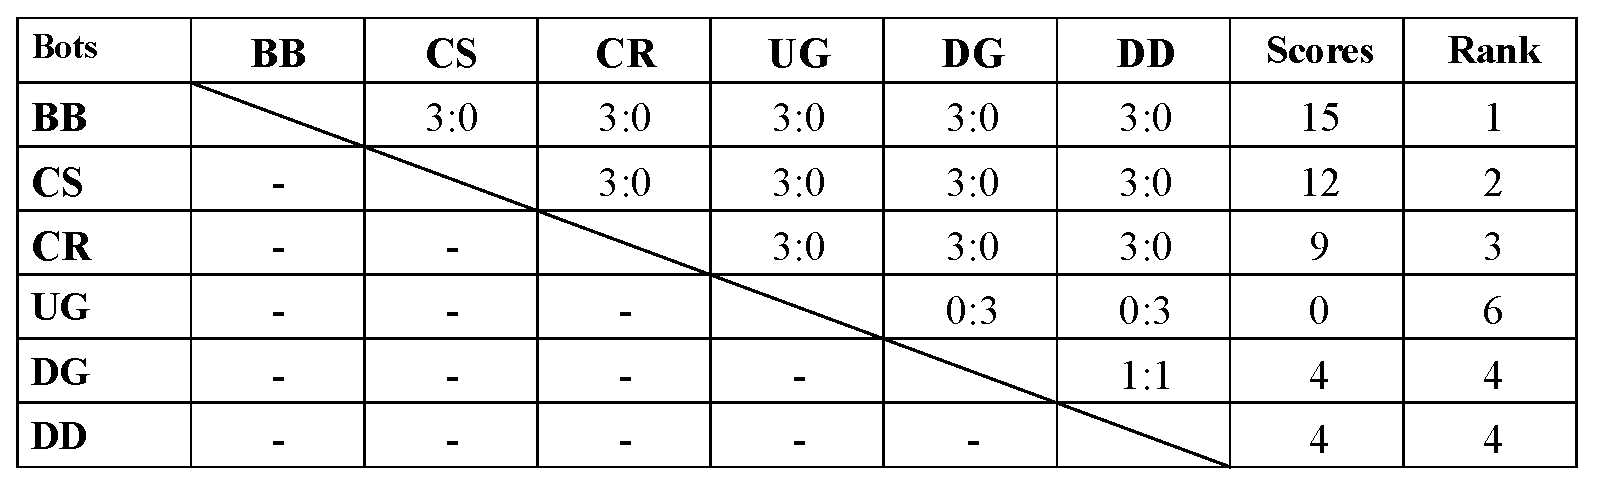
\includegraphics[width=0.7\textwidth]{macro.eps}
%\caption{Scoreboard (Macro) and Rankings of 6-bot Tournament by ChatMatch.}
%\label{fig:macro}
%\end{figure*}

\subsection{Main Results }
\label{sec:main}
In this subsection, we will first present the evaluation results from our automatic metrics, other baselines and human evaluation. 
Then we will analyze the agreement between all automatic evaluation results and human judgments.  
%\subsubsection*{ChatMatch Final results}
%As we can see,  BB scores the top in our scoring framework (both for micro and macro). 
%BB is a competitive bot as it aims at performing well in multiple chitchat test sets in different domains. 
%CS and CR come in second and third respectively. They score quite close to each other as they use the same fine-tuned baseline seq2seq model, which only differ in the 
%choice of specific parameters for some improvement in different aspects. 
%DG and DD score close to each other. UG is always losing the match and ranks at the bottom. 
%We can find an obvious difference between the scores of  
%''the loser'' and the other five bots.

\subsubsection*{Final Scoring of Bots}

\tabref{tab:baseline-scoring} 
shows that BB scores the top among all by our framework. 
It is a well-known competitive bot that performs well in multiple 
chitchat test sets in different domains. 
CS comes in second. 
CS and CR are two controllable neural text generation model 
using conditional training and weighted decoding to control
different attributes.
Here, CS is designed for controlling specifity while CR aims at controlling response-relatedness.
%CS performs quite well in our automatic assesment based on seven dimensions. 
PL, CR, DD and UG score close to each other. 
DG always loses the match and ranks at the bottom.
  
We also show the native scores obtained by using different baseline evalution metrics and human rankings in \tabref{tab:baseline-scoring}. 
We can see that BB ranks the best in Human Rankings. As for two common automatic metrics PPL and TA, CR ranks the best in PPL while UG and DD rank the best in TA. 
BB and PL perform badly according to TA, which is inconsistent with our human evaluation results. PPL can only evaluate whether the sequence generated by the model is close to human language without considering the context. 
%TA reflects whether the generated response matches the ground truth of the dataset. As reasonable responses are not limited to ground truth itself,
% it is difficult to correctly evaluate the ability of the chatbot with static scripts. 
In the process of calculating the CC metric, PL ranks the best. 
We find that CC tends to give a higher score to the shorter response, 
so BB and other chatbots that prefer to generate a longer sequence can not get a reasonable evaluation.
%\KZ{Need more explanations about why we got these automatic results.
%And compared to human, discuss a bit...}

\begin{table}[ht!]
\centering
\scriptsize
%\small
\begin{tabular}{lrrrrrrr}
%\hline
\toprule
& BB &PL& CS & CR & UG & DG & DD  \\ \midrule
PPL & 13.89 &11.64 &10.83 &\textbf{10.74} &16.35 & 20.19 & 14.88  \\
TA & 0.12 & 0.05& 0.12& 0.10 & \textbf{0.23} & 0.19& \textbf{0.23}  \\
CC& 0.47 &\textbf{0.77} &0.61  &0.72 &0.58  & 0.69 & 0.59  \\ 
STB & 2 &\textbf{1} &3 & 7& 6 & 5 & 4\\
CM &\textbf{16}  &8&  15&7 &6& 0& 7\\\midrule
%Micro & \textbf{58}&33 &42 &37 &39 & 25 & 34\\ 
%CMR&\textbf{1} &3&2 &4 &6 &7 &4 \\ 
HR& \textbf{1} &2& 4& 5& 7&6 & 3\\
\bottomrule
\end{tabular}
\caption{Native Scores by Competing Evaluation Methods and 
Average Human Judgments in terms of rankings (HR).}
\label{tab:baseline-scoring}
\end{table}



\begin{table}[th]
\centering
\scriptsize
\begin{tabular}{lccc}
\toprule
 & Overall & Time Efficiency\\ \midrule
PPL  &0.14 & 30 secs \\
TA&-0.42 & 10 secs \\
CC&-0.04 & 1 min\\
STB &0.62 & \textasciitilde 60 min/human\\
Human & -  & \textasciitilde 90 min/human \\
CM&\textbf{ 0.68} & 2 min 57 secs\\
 \bottomrule
\end{tabular}
\caption{Agreement between all evaluation frameworks and 
human judges on
overall performances (Kendall's $\tau$ and workload). }
\label{tab:main}
\end{table}

\tabref{tab:main} shows the final correlation results of the baseline models and our models. 
%However, common automatic evaluation metrics such as PPL and CC present poor agreements 
%with human judgements as their ranking agreement coefficient is close to zero, 
%which indicates a weak agreement. 
%TA is even negatively correlated with human judges. It  reflects whether the generated response matches the ground truth of the dataset. As reasonable responses are not limited to ground truth itself,
% it is difficult to correctly evaluate the ability of the chatbot with static scripts. 
%\textit{Spot The Bot} correlates well with human judgements as they 
%mainly depend on human annotations themselves.
The agreement between our metric and human judgment is 0.68,
 which is even better than the agreement among human judges ( $\tau = 0.53$ ). 
This indicates CM's evaluation results are very close to the average point reaching by ten different human judges. 

\textit{Spot The Bot} correlates well with human judgments as they
mainly depend on human annotations themselves. 

However, common automatic evaluation metrics such as PPL and CC 
present poor agreements with human judgments as their ranking 
agreement coefficient is close to zero,
which indicates a weak agreement.
TA is even negatively correlated with human judges. 
It reflects whether the generated response matches the ground truth of the dataset. As reasonable responses are not limited to ground truth itself,
 it is difficult to correctly evaluate the ability of the chatbot with static scripts.

\subsection{Time Efficiency}
\label{sec:time}
The results about time efficiency is shown in \tabref{tab:main}. 
Compared with human judgments, each human judge takes about 90 minutes on average to complete
the conversations with all 7 bots, decide ratings on seven dimensions and then give their overall ranking.
Meanwhile, our system only requires less than 3 minutes to evaluate all the 7 bots.
 To put it in perspective, we ask three human judges to evaluate the same
7 bots by \textit{Spot The Bot} framework. It takes on average one hour for
each human judge to complete the ranking.

%We also notice a good correlation between ChatMatch's micro scoring metric
%and human judges on Non-repetitiveness dimension as 
%well. However, neither of our two scores fare very well with
%consistency, probably because it is harder for us to 
%detect implicit inconsistencies using our rules while human can better pick up such inconsistencies.
\subsection{Ablation Studies}
\label{sec:ablation}
In this subsection, we exam the effects of different factors
(e.g., number of exchanges, similarity functions, starting utterance, 
scoring methods, etc.) on the final results. 
  

\subsubsection*{Effect of the Starting Utterance}

As most of the chitchat bots we test in the competition 
are for open domain, we provide a list of contexts about 
everyday life as the candidates for the starting utterances, 
which involves greeting, declarative sentence and a question.  
Their performances and simple examples are shown 
in \tabref{tab:multi-context}.

\begin{table}[th!]
\centering
\scriptsize
\begin{tabular}{llr}
%\hline
\toprule
 & Example  & Avg ($\tau$)\\ \midrule
Greetings  & ``Hi! How are you?'' & 0.59  \\
Declarative  & ``I'm not feeling well this morning.'' & 0.62  \\
Question  & ``What did you do last week? '' & \textbf{0.68}  \\
%Average  & & 0.35  \\
\bottomrule
\end{tabular}
\caption{
Agreement with human judgments using different starting utterances.} 
%Average denotes agreement after summing up scores with 
%three different starts.}
\label{tab:multi-context}
\end{table}

 As \tabref{tab:multi-context} shows,
 all three starting utterances lead to a 
good correlation with human. 
The model that starts with a question performs the best since 
raising a question is always a good way to start a conversation 
and make the bots to start talking about it.
%However, we do not find a significant difference with different 
%starting utterance. 
We also find that when two 
bots are free to talk without human intervention, they prefer 
to steer the chat to their ``comfort zones'' (e.g., talking about 
their basic personal information) rather than stick to the ball 
``started'' by CM. 

\subsubsection*{Different Number of Exchanges in a Game} 

We also test CM with different number (e.g., 5, 10, 25, 50, 100, 150 and 200) of exchanges in a game.
A game of 100 exchanges reaches the best agreement between 
CM and human judgments, which we believe is long enough to make the bots
 expose their flaws
and show their strengths.


\subsubsection*{Similarity Functions} 
 We provide a set of simple similarity functions 
to score diversity(non-repetitiveness) and consistency in chat logs which are: 
tf-idf cosine similarity, mean of Word2Vec sentence cosine similarity 
and Bag-of-Word Jaccard coefficient. Agreement using these three functions are 0.68, 0.65 and 0.62 respectively. We choose tf-idf cosine similarity in
the rest of the experiments.

%\begin{table}
%\scriptsize
%\centering
%\begin{tabular}{lcccc}
%\toprule
%&tf-idf & Word2Vec & Jaccard \\ \midrule
%$\tau$ &\textbf{0.68} &  0.65 & 0.62\\
%Time &\textbf{ 2m 57s} &  3m 1s & 5m 52s\\ \bottomrule
%\end{tabular}
%\caption{Comparison of three similarity functions using $\tau$ agreement.}
%\KZ{Run a few times to get average timem then update the number in time efficiency section.}
%\label{tab:similarity}
%\end{table}  

\subsubsection*{Stand-alone Tests of Individual Dimensions}
%\KZ{The purpose of this experiment? Simplify the whole sec.}
Additionally, with the aim of testing the effect of each individual 
scoring dimension
at game level, we set the other dimensions' coefficients to zero
 and compare their agreements with human judges. 
\tabref{tab:stand-alone} shows the agreement with human judges 
and also the best performing bot for each dimension. 
 
\begin{table}[ht!]
\centering
\scriptsize
\begin{tabular}{lrrrrrrr}
%\hline
\toprule
& Flu& Kno& Pro& Spf& Div& Con & Rel \\ \midrule
$\tau$ & 0.15 &-0.10 &0.10 &0.20 &0.52& -0.11 & \textbf{0.68}  \\
Top bot &BB &PL &BB &BB &BB &UG &UG\\
\bottomrule
\end{tabular}
\caption{Stand-alone tests of individual dimension. $\tau$ is agreement with
human judges on each dimension.} 
\label{tab:stand-alone}
\end{table}

Relevance and Diversity have presented a strong agreement with general human judgments. These two dimensions are usually the first two things that come to human judges' mind while completing the evaluation. Bots that generate highly context-related and diverse responses always rank highly in human evaluation.  
Agreements between Specificity, Fluency, Proactivity and human judgments are quite weak since they have less influence on human evaluation, even though they are important abilities for bots to improve.
Knowledge and Consistency are weakly negatively correlated to human judgments. The first main reason for this is that they are often ignored by humans while ranking the bots. Second, our automatic rule-based algorithms can only 
capture some instances of inconsistency and ignorance.
 This kind of inconsistency and ignorance are always common in less capable bots. More potent detection rules will be introduced in the future.

As for the bots which perform the best for each individual dimension,
 according to CM, BB performs the best for Relevance, Diversity, Specificity, Fluency and Proactivity while PL and UG perform the best in Knowledge and Consistency respectively. Besides, UG hardly contradicts itself as it is always repeating something from history.  
\subsubsection*{Choices of Weights for Individual Dimension}

Here we test two sets of weights which are used for summing up individual dimensions at game-level:
\begin{itemize}
\item Identical weight choices: each dimension is worth one point.
\item Fine-tuned weights: we fine-tune seven coefficients with a linear regression model
 according to the rates about three dimensions 
and the overall rankings provided by human judges, we set $fluency = knowledge = diversity = 0.33$, others$=0$.
\end{itemize}

 The final results with these two sets of coefficients are: 
$\tau^i = 0.68, \tau^f = 0.14 $ respectively. 
It is not surprising to find weak agreement between our framework with fine-tuned weights and human judgments as 
humans' standards for individual dimension rating are usually rather ambiguous according to \tabref{tab:inter}. As a result, inter-agreement among human judges on individual dimension is quite weak and the parameters fine-tuned based on this relationship are no longer reliable.

 As identical weight choices perform better, we decide to keep using the identical weight set in other part of our experiments.  
 
\subsubsection*{Points for a Win, Tie and Lose at Match Level Scoring}
We have tried three sets of points a bot will gain aften a win, tie or lose at match-level:
\begin{itemize}
\item win = 3, tie = 1, lose = 0
\item win = 1, tie = 0, lose = -1
\item win = 1, tie = 0.5, lose = 0
\end{itemize}

With these three sets of parameters, 
we get 0.68, 0.62 and 0.62 as agreement with human judgments respectively, which indicates little effect on final results.

%\subsection{Time Efficiency}
%\label{sec:time}
%As for timing, a human judge takes more than 90 minutes on average to complete 
%the conversations with all 7 bots, decide ratings on seven dimensions and then rank the bots. 
%Our system only requires about 2 min 57 secs on average to 
%complete a game, 
%which is an 100-exchange conversation. As all 42 games can be processed in 
%parallel, the total time cost for evaluating all the 6 bots is less than
%3 minutes. To put it in perspective, when we evaluate the same
%6 bots by \textit{Spot The Bot} framework, it takes on average one hour for
%each human judge to complete the ranking.


\subsection{Response Diversity of Direct Chats Between Bots}
\label{sec:diversity}
While going through direct bot-bot chat logs, we find that sometimes bots 
are better conversation partners than humans. 
To demonstrate these findings, 
we calculate the average specificity score for chat logs between 
CR and human annotators.  Then we compare the results with the 
average specificity score for chat logs between CR and PL as 
\tabref{tab:div} shows. We can see that CR tends to generate longer 
responses with richer vocabulary use while being faced with PL than 
talking to a human judge.    

\begin{table}
\scriptsize
\centering
\begin{tabular}{lccccc}
\toprule
& D-1 & D-2 & avg(D-1, D-2)&Avg Len\\ \midrule
CR(human) & 0.52  & 0.86   &0.69  &7.2 \\ \midrule
CR(PL) & 0.52  &\textbf{ 0.90}    &\textbf{0.71} &\textbf{8.9} \\ \bottomrule
\end{tabular}
\caption{Distinct-1/2 and average length of response for bot-bot chat logs and human-bot chat logs. }
\label{tab:div}
\end{table}

%\subsection{Discussion}
%In our experiments, we only test chatbots used for daily chatting. 
%It would also be useful to test chatbots from other domains 
%(e.g., domain-specific bots with specialized knowledge, 
%empathetic bots used for entertainment, etc.) in the future.  
%In order to detect more subtle weakness in bots, we probably 
%need a more comprehensive setup for future design of the system . 

